\section{Hand Motion Dimensionality}

At the core of our technique is the assumption that hand motion is relatively low-dimensional.  Even though a full resolution skeleton of the hand can have several dozen degrees of freedom (DOF), many of the DOFs of the hand show correlations, so that the inherent dimensionality of the hand motions is much lower ~\cite{SanFlaSoe98,BraZha04,JoeOSu09}. In our approach, PCA is used to exploit this low dimensionality as we assume that PCA will allow us to capture the important features of the whole-body hand motion in a small number of principle components.  
%Further, we assume that if we record markers that well-inform these \emph{key} principle components, we can estimate the DOFs of the whole hand.

To support these assumptions, we performed various tests to exploit the power of PCA for hand animation. First, we use PCA on the marker positions of our reference data. The dimensionality of this principle component representation is 39, comprised of 3 root-corrected position values for each of the 13 markers.  \emph{XXX It would be nice to have something here such as 80\% of the information can be explained through the first three components.}
We show that joint angles alone are not capable of producing the reconstructions we realize through PCA in Figure~\ref{}. 

\begin{figure}
  \centering
  %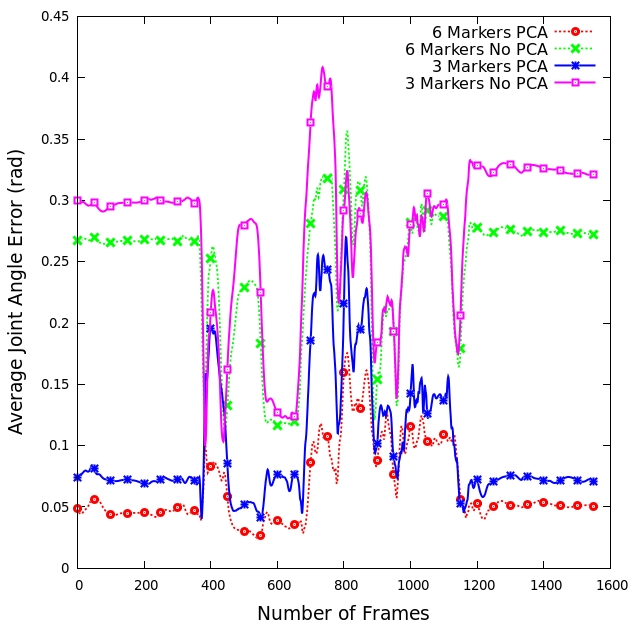
\includegraphics[height=3cm]{images/avgError_6_3_jangles_babySigns1.jpg}
  %\caption{{\label{fig:avgError}}PCA vs. Joint angles.}
\end{figure}

% the paragraph below seemes to already say what belongs in Sections 4 and 5
PCA identifies the most important information in this database by making it the first component. Each subsequent component is less valuable than its predecessor. Using this knowledge, we sum up the values of each component over all of the samples and weigh each sum based on importance (which component). Each weighted sum correlates with a marker, and the markers are then ordered in terms of importance by their weighted sum. The chosen marker set is then used for the data we wish to reconstruct. 
To reconstruct a sequence of motion, we first only use data from the marker set selected in the previous step. This is the equivalent of having our performer only wear these markers in the initial capture session. These marker position are plugged into our regression model to determine the full motion of our low dimensional sequence in principle component space.

Second, starting again with our reference database, we conduct a PCA over the joint angles of the hand motion. With 18~joints with 3 Euler angles each, this results in a new principle component representation of the joint angles with 54 components. We performed an analysis to judge the ability of the PCA to directly reconstruct the original database motion and found that with as few as ten components the PCA could produce a motion with small but acceptable visual artifacts. % again, here, would be nice to say something like: 80% of the information can be explained with the first 3 components
An error plot of the reconstruction error measured by the joint angle deviation from the synthesized motion and the original motion appears in Figure~\ref{}.  Similar findings are reported using a small set of components from PCA to encapsulate the motion of full-body motion~\cite{SafHodPol04} and our results here support similar observations made over hand motions.

\begin{figure}
  \centering
%  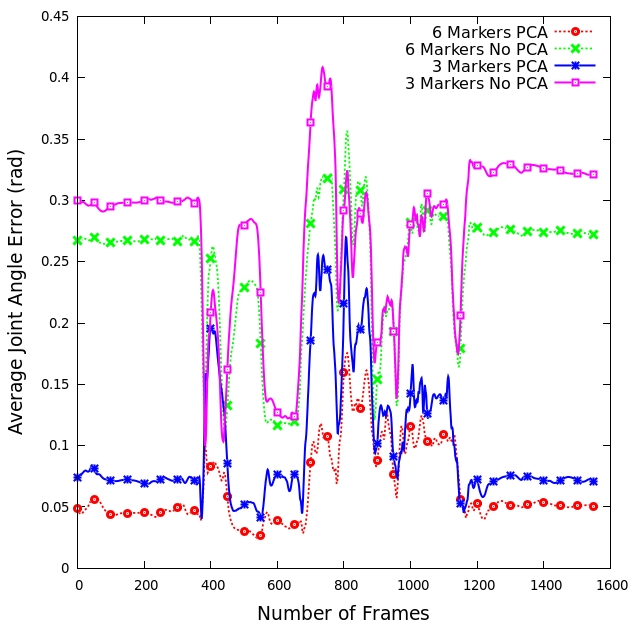
\includegraphics[height=4cm]{images/avgError_6_3_jangles_babySigns1.jpg}
 % \caption{{\label{fig:avgError}}PCA vs. Joint angles.}
\end{figure}

